\section{What the Household Loses and What It Does}\label{sec:household}

\subsection{The father's earnings and the family's income}

Table~\ref{tab:displacement_family} reports the mean effects of the father's displacement over years 1 to 3 after the
job loss, and Figure~\ref{fig:displacement_es} the effects year by year. The job loss is a large and lasting shock.
His hours fall by about 300 in the year of the job loss and recover within four to five years, but his labor income
stays about \$6,000--7,000 a year lower six years later. Over years 1 to 3, his labor income falls by \$4,160 for Black
fathers and \$9,622 for White fathers, about 17\% and 24\% of their pre-displacement labor income. Family income falls by
at least as much (by \$4,832 and \$11,179), so on average none of the loss is made up within the household. Displaced
fathers' earnings were already lower in the year before the job loss (by \$2,821), the dip before displacement that
\citet{jacobson1993earnings} document. It is a fall in hourly earnings, not hours ($-\$1.01$ an hour, while hours
change by $-15$, $p=0.477$), it appears in the reports that carry the year of the job loss rather than in those dated
by assumption, and it is largest before plant closures, as expected of declining employers.\footnote{Code: \texttt{IGE/19.FatherDisplacement.py}, \texttt{IGE/20.PaperDisplacement.py}. Closures-only
versions of every outcome: \texttt{output/father\_displacement.md}, Section 2c.}

\begin{table}[htbp]\centering\small
\caption{The father's displacement and the family}\label{tab:displacement_family}
\resizebox{\textwidth}{!}{%
\begin{tabular}{lcccccccc}
\toprule
 & \begin{tabular}[b]{@{}c@{}}(1) Father's\\hours\end{tabular} & \begin{tabular}[b]{@{}c@{}}(2) Father's\\labor income\end{tabular} & \begin{tabular}[b]{@{}c@{}}(3) Family\\income\end{tabular} & \begin{tabular}[b]{@{}c@{}}(4) Wife's\\hours\end{tabular} & \begin{tabular}[b]{@{}c@{}}(5) Wife\\employed\end{tabular} & \begin{tabular}[b]{@{}c@{}}(6) Still\\with wife\end{tabular} & \begin{tabular}[b]{@{}c@{}}(7) AFDC/TANF\\\end{tabular} & \begin{tabular}[b]{@{}c@{}}(8) Food\\stamps\end{tabular} \\
\midrule
\multicolumn{9}{l}{\textit{A. All fathers}} \\
Displaced, years 1--3 & $-145^{***}$ & $-8,037^{***}$ & $-9,345^{***}$ & $51^{**}$ & $0.008$ & $-0.031^{***}$ & $0.008$ & $0.036^{***}$ \\
 & (22) & (748) & (960) & (23) & (0.013) & (0.008) & (0.005) & (0.010) \\
Displaced / control fathers & \multicolumn{8}{l}{2,417 / 63,669} \\
\multicolumn{9}{l}{\textit{B. Black fathers}} \\
Displaced, years 1--3 & $-146^{***}$ & $-4,160^{***}$ & $-4,832^{***}$ & $40$ & $0.026$ & $-0.045^{***}$ & $0.010$ & $0.042^{**}$ \\
 & (35) & (757) & (1,082) & (38) & (0.019) & (0.015) & (0.009) & (0.019) \\
Displaced / control fathers & \multicolumn{8}{l}{989 / 17,746} \\
\multicolumn{9}{l}{\textit{C. White fathers}} \\
Displaced, years 1--3 & $-130^{***}$ & $-9,622^{***}$ & $-11,179^{***}$ & $59^{**}$ & $-0.002$ & $-0.019^{**}$ & $0.007$ & $0.033^{***}$ \\
 & (28) & (1,071) & (1,353) & (30) & (0.018) & (0.009) & (0.006) & (0.010) \\
Displaced / control fathers & \multicolumn{8}{l}{1,428 / 45,923} \\
\multicolumn{9}{l}{\textit{D. Youngest child aged 0--5}} \\
Displaced, years 1--3 & $-158^{***}$ & $-7,733^{***}$ & $-8,052^{***}$ & $112^{***}$ & $0.041^{**}$ & $-0.030^{***}$ & $0.012^{*}$ & $0.039^{***}$ \\
 & (29) & (976) & (1,127) & (31) & (0.018) & (0.010) & (0.007) & (0.013) \\
\multicolumn{9}{l}{\textit{E. Youngest child aged 6--17}} \\
Displaced, years 1--3 & $-149^{***}$ & $-9,686^{***}$ & $-11,768^{***}$ & $-26$ & $-0.038^{**}$ & $-0.030^{**}$ & $0.002$ & $0.032^{**}$ \\
 & (34) & (1,118) & (1,600) & (36) & (0.018) & (0.012) & (0.008) & (0.014) \\
\bottomrule
\end{tabular}}
\begin{minipage}{0.95\textwidth}\footnotesize Stacked event study of a father's first displacement (plant closed or moved, laid off or fired, from the PSID question on why the last job ended), with clean controls (fathers not displaced up to six years after the event year). Coefficient: mean of the event-time effects at years $+1$ to $+3$, relative to year $-2$. Fathers are male heads with a child aged 0--17 and positive hours at baseline; SRC and SEO samples, Black and White, unweighted. Incomes in 2000 dollars; wife's outcomes for the wife present at baseline. Standard errors clustered by 1968 family. *** $p<0.01$, ** $p<0.05$, * $p<0.1$. Source: \texttt{IGE/19.FatherDisplacement.py}.\end{minipage}
\end{table}


\begin{figure}[htbp]\centering
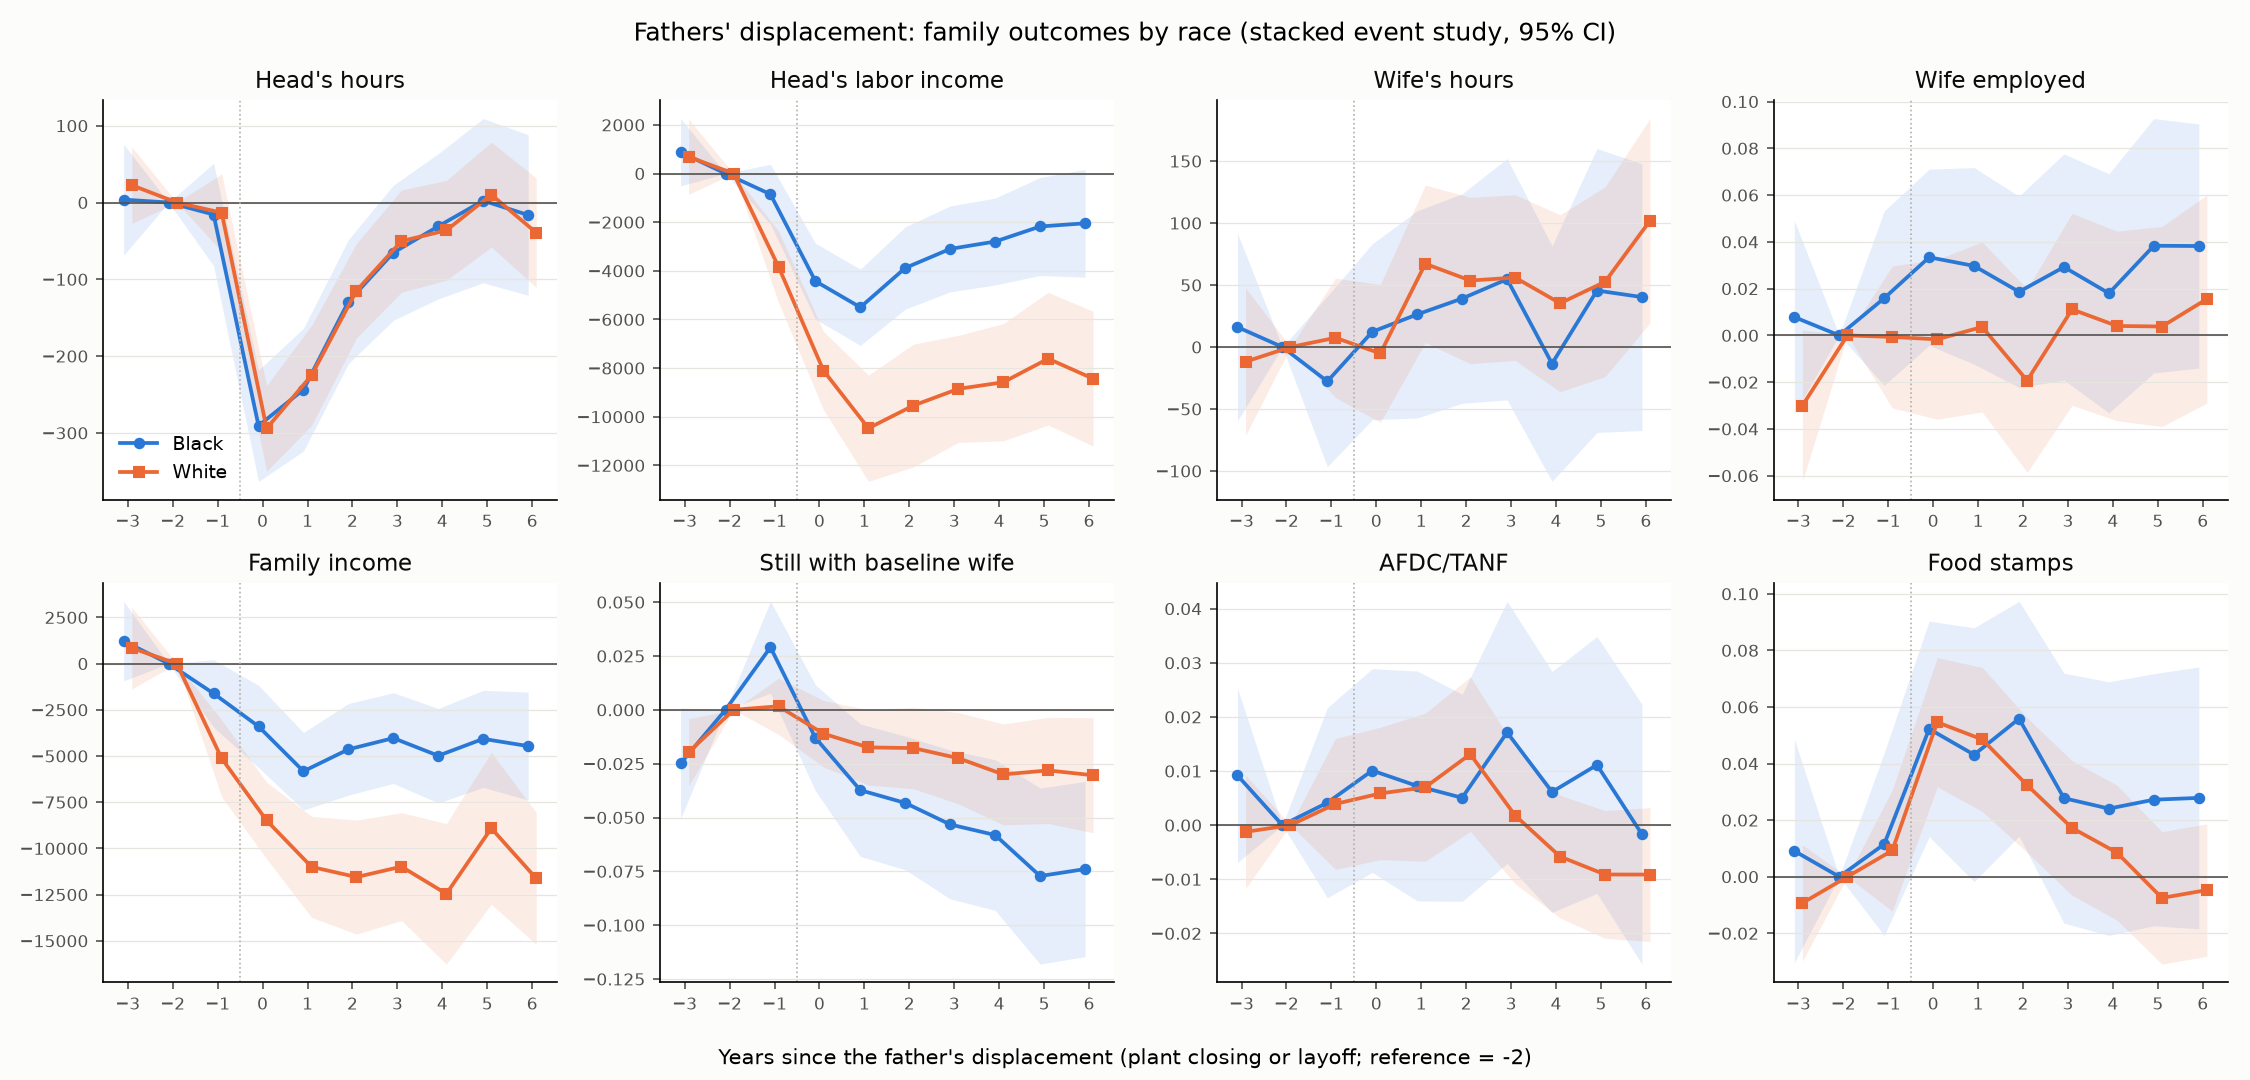
\includegraphics[width=\textwidth]{father_displacement_es.png}
\caption{The father's displacement and the family, by race (PSID)}\label{fig:displacement_es}
\begin{minipage}{0.95\textwidth}\footnotesize Stacked event study, effects by year relative to the displacement
(reference year $-2$), with 95\% confidence intervals; Black and White fathers. Sample and controls as in
Table~\ref{tab:displacement_family}.\end{minipage}
\end{figure}

\subsection{The wife's response: search at once, jobs slowly}

Wives make up a small part of the loss, and mainly when the children are young. On average, a wife works 51 more hours
a year after her husband's job loss, and her employment does not change. When the youngest child is under six, she
works 112 more hours and is 4.1 percentage points more likely to be employed; when the youngest child is of school age,
her hours do not rise and her employment falls by 3.8 points. Black wives respond less than White wives when the
children are young: 68 more hours, not significantly different from zero, against 117 for White wives.

The monthly CPS shows how the response unfolds. Wives who were not working when their husband lost his job begin to
look for work at once: their probability of being unemployed and looking rises by 8.8 points in the month after his job
loss (0.088$^{***}$, on a base of 6.0\%). Jobs come slowly: their probability of being employed rises by 2.2 points after
one month, 4.2 points after three and 4.0 points after twelve (all $p<0.001$). The response is concentrated among
mothers of young children (3.6 points after one month, against 0.4 for wives without children, $p=0.382$) and is larger
for Black wives (4.7 points after one month and 10.0 after twelve, against 1.8 and 3.4 for White wives). Wives who were
already unemployed when their husband lost his job become less likely to find work ($-0.020^{*}$ after one month,
$-0.050^{**}$ after three): their own labor market has been hit too. The SIPP, which follows wives for three years, shows the same
pattern over a longer horizon (Figure~\ref{fig:sipp_wife}): among wives with no job the month before, employment
builds up over about six months, from 1.9 points in the month of the husband's separation to 5.4 points after six
months, and stays about 4.4 points higher after two years. These wives were already more often looking for work before
his separation (4.4 points in the month before), so the SIPP's rise in looking at the separation is small (to 5.3
points); the CPS, which records search in the reference week, shows the jump. Because wives who were working lose their
own jobs in the same months, the net change in all wives' employment is about zero for a year
(Appendix~\ref{app:robust}). The
PSID's annual interview-week status does not show a rise in looking for work a year after the job loss (for all wives $-0.001$, s.e.\ 0.008), because by then the search
spell has ended in a job or in leaving the labor force; the annual snapshot misses what the monthly data show.

\begin{figure}[htbp]\centering
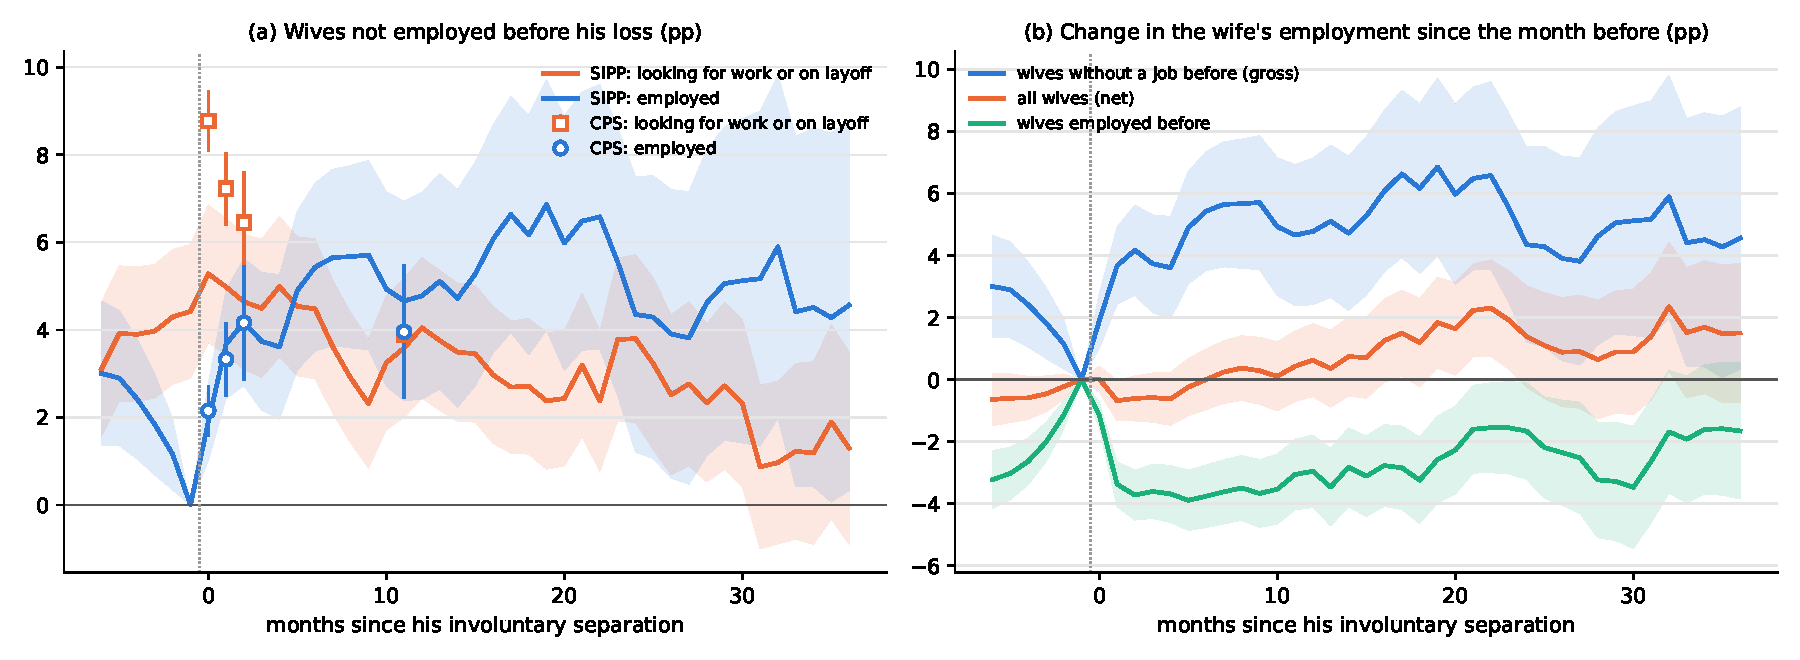
\includegraphics[width=\textwidth]{fig_sipp_wife_response.pdf}
\caption{The wife's response month by month (SIPP and CPS)}\label{fig:sipp_wife}
\begin{minipage}{0.95\textwidth}\footnotesize (a) Wives with no job in the month before the husband's involuntary
separation: difference in the probability of being employed and of looking for work or being on layoff between wives
whose husband separates in month 0 and wives whose husband stays employed, by month (one linear probability model per
month, base panel $\times$ month fixed effects; SIPP 2004, 2008 and 2014 panels). Employed at $s=0$: 1.9$^{***}$
points (s.e.\ 0.5); $s=6$: 5.4$^{***}$ (1.0); $s=24$: 4.4$^{***}$ (1.6, $p=0.007$). Looking: 4.4$^{***}$ (0.8) at $s=-1$, 5.3$^{***}$
(0.8) at $s=0$. Markers: CPS basic monthly 1994--2023, wives not employed in month $t$, husband's job loss at $t+1$,
plotted at $s=k-1$ for $t+k$; state $\times$ month fixed effects; looking at $t+1$: 8.8$^{***}$ (0.4); employed at
$t+3$: 4.2$^{***}$ (0.7) and at $t+12$: 4.0$^{***}$ (0.8). (b) Change in the wife's employment since the month before
his separation: wives without a job before (gross entry), all wives (net) and wives employed before (their own job
loss). 95\% confidence intervals clustered by household. Code: \texttt{40.SIPPJointLoss.py},
\texttt{37.CPSJointLossChecks.py} (\texttt{output/sipp\_joint\_loss.csv}, \texttt{output/cps\_joint\_loss\_checks.csv}).
\end{minipage}
\end{figure}

\subsection{Gross and net added work}

The joint job loss changes how the added-worker response should be read. Average estimates of the added-worker effect
\citep{stephens2002worker, halla2020job} net two groups of wives: those who work more after their husband's job loss and
those who lose their own job with his. The PSID allows the two to be separated from 1984 on, when wives' own job-end
reports begin. Splitting displaced families by whether the wife was herself displaced in the three years around the
husband's job loss, the gross response of wives who kept their jobs is 47 hours a year over years 1 to 3 ($p=0.165$),
and 97 hours when the youngest child is under six ($p=0.032$). Wives who were displaced with their husband work 388
fewer hours ($p=0.003$). Because 10.6\% of the wives of displaced men are displaced themselves, against 5.0\% of the
wives of other men, the joint losses offset 35 hours of the gross response (s.e.\ 14; $p=0.013$), so the net response in
these years is 12 to 16 hours and not significant (Figure~\ref{fig:gross_net}).\footnote{Interaction model in the
stacked event study, event years 1984--2021; the wife's own displacement is observed for 82\% of displaced families
(it is missing when the couple has split or is not interviewed), and conditioning on it is descriptive. The offset
rests on 119 displaced husbands whose wife was also displaced. The average response of 51 hours in
Table~\ref{tab:displacement_family} combines events before 1984 (74 hours, $p=0.029$), when the wife's own job losses
are not measured, with events from 1984 (30 hours, $p=0.364$). Code: \texttt{IGE/38.PSIDJointLossChecks.py}
(\texttt{output/psid\_joint\_loss\_checks.md}).} The joint losses remove more than two thirds of the gross response of
the average wife. The small net response reflects, in large part, not an unwillingness or inability to add work but the
loss of the wife's own job to the same shock. A model of household insurance in which the second earner's job is
independent of the first earner's, or in which only the net response is targeted, overstates what the family can
absorb in the months of the shock.

\begin{figure}[htbp]\centering
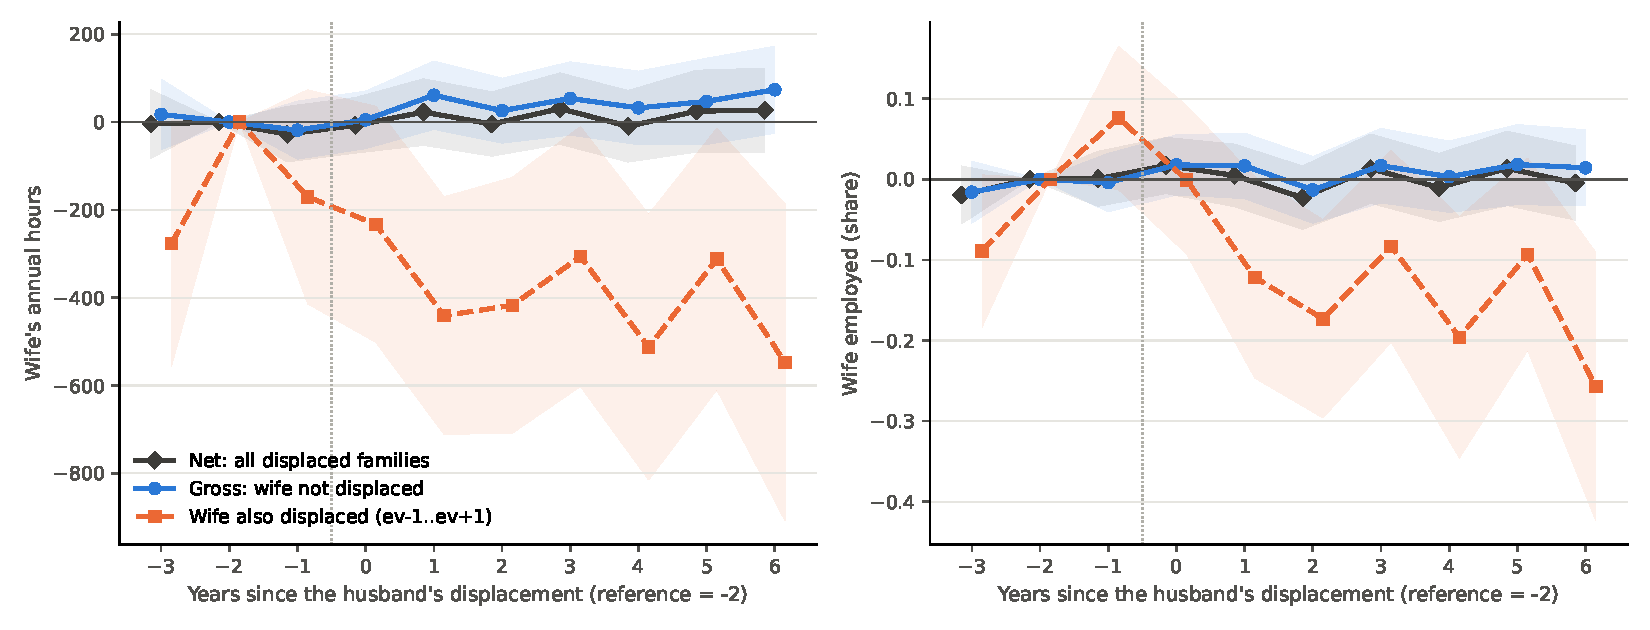
\includegraphics[width=0.85\textwidth]{fig_gross_net_awe.pdf}
\caption{Gross and net added work after the husband's displacement (PSID, 1984--2021)}\label{fig:gross_net}
\begin{minipage}{0.95\textwidth}\footnotesize Wife's annual hours (left) and employment (right) by year relative to the husband's displacement,
for displaced families in which the wife kept her job (gross response), in which she was displaced too, and all
displaced families (net response), relative to control families; 95\% confidence intervals clustered by 1968 family.
Code: \texttt{IGE/38.PSIDJointLossChecks.py}.\end{minipage}
\end{figure}

\subsection{The wife's own labor market and the difference by race}

Beyond the joint job loss, the wife's own labor market at the time of the husband's job loss does not limit her
response: employment growth in her sector, labor demand in her state and the change in her state's unemployment rate do
not weaken it. The racial difference in the response lies among wives who were not working before the husband's job
loss, who enter work after it if they are White and much less if they are Black, although Black wives search more in
the CPS. Black spouses are slightly less alike in industry than White spouses, and joint job losses are equally
frequent, so correlated shocks do not explain this difference. A search friction that is higher for Black women and
preferences, including the value of time with young children, remain as explanations; the model separates them by
their implications for women's search and employment over the life cycle.

\subsection{The marriage}

The job loss also strains the marriage. The share of displaced fathers still living with the wife they had before the
job loss falls by 4.5 percentage points over years 1 to 3 for Black fathers and by 1.9 points for White fathers, and the
gap keeps widening: by year 6 it is 7.4 points for Black fathers (s.e.\ 2.1) and 3.0 points for White fathers (s.e.\
1.4). The divorce response to job loss is known \citep{charles2004job}. The point estimates are about twice as large
for Black as for White fathers, but the racial difference is not statistically significant, and with plant closures
only the response is similar to that after layoffs (Black $-0.044$, $p=0.108$, against $-0.044^{**}$ after layoffs;
White $-0.015$, $p=0.304$, against $-0.021^{*}$), so the distinction between layoffs and closures that
\citet{charles2004job} find does not appear here.\footnote{Closures-only and layoffs-only versions of every outcome of
Table~\ref{tab:displacement_family}, by race and by child age: \texttt{output/psid\_joint\_loss\_checks.md},
Section 2. With closures only, wives' hours rise by 83 ($p=0.040$), and by 210 when the youngest child is under six
($p<0.001$).}

The wife's own job loss strains the marriage as much, as \citet{charles2004job} found, and their result for wives
that layoffs matter and plant closings do not reappears here. With the roles reversed, so that the event is the wife's first
displacement (wives of male heads with children who worked before; events 1984--2021), the probability that she is
still with the husband she had before falls by 4.6 percentage points over years 1 to 3 ($-0.046^{***}$, s.e.\ 0.012)
and by 9.0 points over years 4 to 6 ($-0.090^{***}$, s.e.\ 0.016), among 1,205 displaced wives; by 4.8 points for Black
wives ($p=0.037$) and 4.0 points for White wives ($p=0.005$), a difference of 0.008 ($p=0.77$). Her hours fall by 127 a
year over years 1 to 3 and are back by years 4 to 6, while the gap in the marriage keeps widening. Estimated in one
regression with the husband's displacement over the same event years, the two responses do not differ ($-0.046$
against $-0.036$ over years 1 to 3, difference $p=0.54$; $-0.090$ against $-0.051$ over years 4 to 6, $p=0.061$). In
three of five of these break-ups it is the husband who leaves the family. A joint loss, both spouses displaced within a
year, gives the largest response: over the six years after the husband's displacement, the share still together is 9.5
points lower when his wife lost her job too ($-0.095^{***}$, $p=0.009$) and 4.1 points lower when she kept hers
($-0.041^{***}$); with 174 joint events the difference is not statistically significant ($p=0.15$). The response
survives baseline characteristics interacted with event time ($-0.033^{***}$ over years 1 to 3), dropping the couples
who lost both jobs, and requiring that both displaced and control wives be interviewed when the job loss would be
reported ($-0.050^{***}$). Two caveats remain. As for the husband's displacement, the outcome equals one before the
job loss by construction, so there is no pre-period placebo. And plant closures alone give a smaller response that is
not significant ($-0.027$, $p=0.19$, 376 closures; layoffs and firings $-0.056^{***}$), and displaced wives were
younger and in shorter marriages than the controls, so part of the response after layoffs and firings may reflect who
is laid off.\footnote{Code: \texttt{IGE/64.SeparationUIAndHerLoss.py} (main estimates) and
\texttt{IGE/65.HerLossRobustness.py} (checks); output \texttt{output/her\_loss\_robustness.md}. Same stacked design
as Table~\ref{tab:displacement_family}, standard errors clustered by 1968 family; events include her own reports as a
female head after a separation, so they are not conditioned on staying married. Her versus his, both designs stacked
in one regression with one clustered covariance; among couples in which both worked before, $-0.044^{***}$ against
$-0.043^{***}$ (difference $p=0.95$). Closures minus layoffs over years 1--6: wife 0.049 ($p=0.082$), husband 0.025
($p=0.33$); with baseline controls, closures $-0.021$ ($p=0.31$). Baseline balance (displaced minus control within
stacks): she is 2.1 years younger, her earnings are \$7,149 lower and his \$10,062 lower, 13 points more of the
couples have been observed together for two years or less (all $p<0.001$); her share of the couple's earnings is the
same ($-0.009$, $p=0.24$); her hours and earnings show no trend before the event (earnings at $e=-3$ and $e=-1$: 455,
$p=0.50$; $-425$, $p=0.39$). Dropping the 244 wives whose husband was displaced within a year of her: $-0.049^{***}$
(years 1--3), $-0.081^{***}$ (4--6); joint against her loss alone over years 1--6, $-0.083^{**}$ against $-0.070^{***}$
(difference $p=0.74$); in the husband's design, joint $-0.095^{***}$ against his loss alone $-0.041^{***}$
(difference $p=0.15$, 174 joint events). By her share of the couple's earnings (above or below the median of 0.36, or
0.40), the responses do not differ ($p \geq 0.33$), although her hours fall by 270 when her share was above the median
and not at all below it. Who leaves (no reason for a separation is recorded): the husband moves out in 60\% of first
separations after her displacement and 65\% among controls, she moves out in 15\% and 16\%, and his death plays no part
($-0.002$, $p=0.44$). Requiring both groups to be interviewed at the first interview after the event year (a displaced
wife must be to report the job loss) makes later attrition equal (0.011, $p=0.36$); filling the outcome from his side
when she is not interviewed then gives $-0.051^{***}$.}

The insurance that survives the marriage is hit as well. A separated mother with children receives \$132 (Black) or
\$327 (White) a month in child support on average; when her husband had been displaced in the two years before the
separation, she receives \$116 a month less ($-116^{***}$, $p<0.001$; Black $-88^{***}$, White $-155^{***}$), and her
food-stamp receipt is 11.4 points higher ($+0.114^{***}$). The father's job loss that precedes the break-up also cuts
the transfer that is meant to replace his earnings after it.\footnote{PSID mothers whose marriage ended in 1984--2020
(marriage-history dates), seen married with a child under 18 in the three years before the separation, aged 25--59;
570 Black and 924 White mothers; outcomes in the ten years after the separation while single. Standard errors
clustered by 1968 family. The comparison with mothers whose husband was not displaced is descriptive. Remarriage is
not lower after his displacement (0.000, $p=0.94$). Code: \texttt{IGE/76.SeparatedMothers.py}; output
\texttt{output/separated\_mothers.md}.}

\subsection{Consumption}

Consumption is measured in the PSID from 1999, so this evidence covers 1999--2021 only. I construct the measure of
\citet{blundell2016consumption}---nondurable goods and services, with a rent equivalent of 6\% of the house value for
owners---for every wave from 1999 to 2021; for 1999--2009 it reproduces their series exactly.\footnote{Items are found in
each wave by their PSID labels; question changes (heating, health insurance premiums, health spending, car repairs,
time units) are harmonised, a combined gas and electricity bill asked from 2007 is added to utilities, and the
categories added in 2005 (clothing, trips, recreation, home repairs, furnishings) are excluded from the consistent
series. Stacked event study as in Table~\ref{tab:displacement_family}, events 2000--2020, event time in interview waves;
standard errors clustered by 1968 family. Code: \texttt{IGE/47.PSIDConsumptionEvent.py}
(\texttt{output/psid\_consumption\_event.md}).} Among 548 displaced husbands, 63 of whose wives were displaced in the
three years around his job loss, consumption barely falls after the husband is displaced alone: by 1.3\% over the first
three interviews after the job loss ($p=0.49$) and 3.2\% at the first ($p=0.13$). After a joint displacement it falls by
7.1\% ($p=0.31$); the difference from a single displacement is $-0.059$ (s.e.\ 0.073, $p=0.42$), $-0.127$ excluding housing
($p=0.14$) and $-0.170$ for food ($p=0.13$) (Figure~\ref{fig:consumption}). Because the wife's job loss can precede her
husband's, the last interview before his job loss can already follow hers; measured against the interview before
that, consumption falls by 21.4\% after a joint displacement ($p=0.025$) and by 18.5 points more than after a single one
($p=0.058$), on 26 joint events. The household's consumption is well insured against the husband's job loss alone; the
point estimates indicate a larger fall when both earners are lost, but with 63 joint events in two-year interview data
the difference is not precisely estimated, as in the panel of \citet{blundell2016consumption}. The model uses the
consumption response to a single displacement as a target for 1999--2021 and the joint-minus-single difference as a
target with its standard error.

\begin{figure}[htbp]\centering
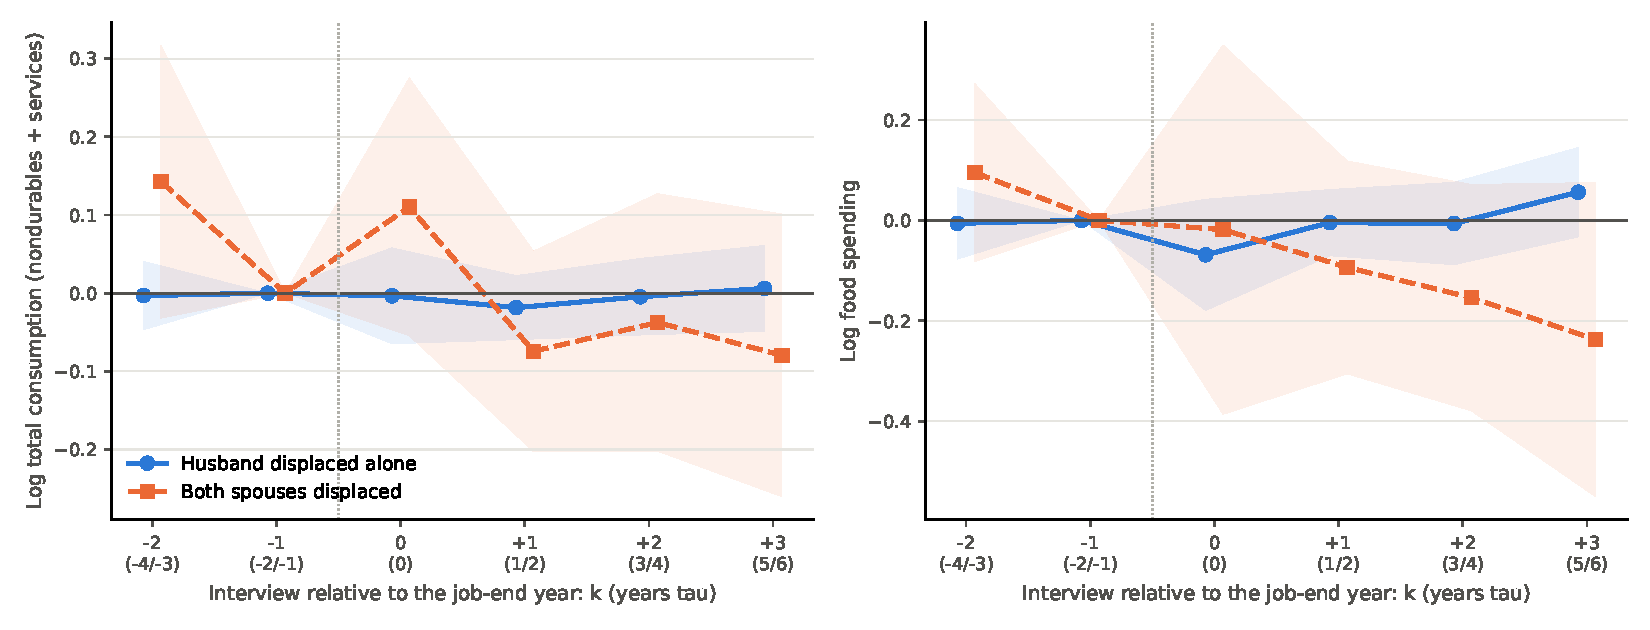
\includegraphics[width=\textwidth]{fig_consumption_single_joint.pdf}
\caption{Consumption around single and joint displacements (PSID, 1999--2021)}\label{fig:consumption}
\begin{minipage}{0.95\textwidth}\footnotesize Log total consumption (nondurables and services, left) and log food
spending (right) by interview relative to the husband's job-end year, for husbands displaced alone and couples in which
both spouses were displaced, relative to couples without a displacement (reference: the last interview before the job
loss); 95\% confidence intervals clustered by 1968 family. Code: \texttt{IGE/47.PSIDConsumptionEvent.py}.\end{minipage}
\end{figure}

\subsection{The safety net}

Food stamp receipt rises by 4.2 points for Black and 3.3 points for White families after the father's displacement,
while AFDC/TANF receipt barely moves. The joint job loss determines which programs can respond, and the monthly SIPP
shows how. When the husband loses his job alone, unemployment insurance reaches him at once: his receipt rises by 23
points in the first three months and stays 13 points higher half a year later, and the couple almost never goes
without both earnings and benefits (1.0\% of couple-months in the first half year). When the wife loses her job too,
his benefits rise by about as much, hers rise by 11 to 18 points, and yet 9.3\% of the couple-months in the first half
year have no earner and no unemployment insurance, 5.7 points more than after his loss alone.\footnote{SIPP panels
2004, 2008 and 2014 (reference months 2003--2016): dual-earner couples with the wife aged 25--59, both employed in
the month before the husband's involuntary separation (layoff, closure, discharge or end of a temporary job) at
$s = 0$; a joint loss is an involuntary separation of the wife in $s = -3, \dots, +3$ (206 events, against 2{,}644
losses of his alone). Clean controls: 29{,}899 couples with a pseudo-event month in which both work and neither
spouse separates involuntarily nearby. Regressions on event month $\times$ group with couple and panel $\times$
rotation $\times$ calendar-month fixed effects, reference $s = -3, \dots, -1$, standard errors clustered by household
(32{,}109 clusters, $N = 516{,}624$). His UI receipt: $+22.6^{***}$ points (s.e.\ 0.7) in $s = 0$--$2$ and
$+13.3^{***}$ (0.7) in $s = 6$--$11$ after his loss alone; $+18.2^{***}$ (2.5) and $+9.7^{***}$ (2.5) after a joint
loss. Her UI receipt after a joint loss: $+10.9^{***}$ (2.1) in $s = 0$--$2$ and $+18.0^{***}$ (2.7) in $s = 3$--$5$.
No earner and no UI: $+6.2^{***}$ (1.4) and $+6.4^{***}$ (1.7) after a joint loss, $+0.5^{***}$ (0.1) and
$+0.7^{***}$ (0.2) after his loss alone; joint minus alone $+5.7^{***}$ (1.7; $p<0.001$) in $s = 3$--$5$ and
$+2.6^{*}$ (1.3; $p=0.055$) in $s = 6$--$11$. Receipt is from the core-wave program items (2004/08: state UI ER05 /
T05AMT, household food stamps THFDSTP, own receipt and coverage ER27, RCUTYP27; 2014: EUC1--3MNYN, RFSYN, RFSCOV).
The employment pre-trend ($-5.9^{***}$ in $s = -6$ to $-4$) follows from requiring both spouses to work at $s = -1$
(\texttt{IGE/78.SafetyNetJointLoss.py}).} In the couple-months of a joint loss in which neither spouse works, which
are a quarter of the first half year, 39\% receive unemployment insurance for neither spouse and 23\% receive neither
unemployment insurance nor food stamps.\footnote{Couple-months $s = 1$--$6$ after a joint loss with both spouses
not employed: 24.0\% of the joint-loss couple-months (1.5\% after his loss alone); among them UI for neither spouse
38.7\%, food stamps 33.8\%, neither program 23.5\% (316 couple-months). After his loss alone, among couple-months with
him not employed: UI for neither 51.2\%, food stamps 9.7\% (6{,}458 couple-months). Weighted by the wife's weight in
$s = -1$ (\texttt{IGE/78.SafetyNetJointLoss.py}).}

Food stamps respond less than the joint loss would suggest, because the couples who lose both jobs are already the
couples on the program. In the three months before his loss, 19\% of joint-loss couples receive food stamps, against
5.9\% of couples in which he loses his job alone and 3.2\% of the controls; receipt then rises by 1.0 to 1.5 points after
his loss alone and by 1 to 3 points, imprecisely, after a joint loss. AFDC/TANF does not move in either
group.\footnote{Food stamp receipt relative to $s = -3, \dots, -1$: after his loss alone $+1.05^{***}$ (0.26) in
$s = 0$--$2$, $+1.51^{***}$ (0.36) in $s = 3$--$5$, $+1.40^{***}$ (0.43) in $s = 6$--$11$; the amount rises by
\$3.9--5.2 a month (2000 dollars, zeros included). After a joint loss $+1.14$ (1.25; $p=0.361$), $+3.28$ (2.23;
$p=0.141$), $+3.26$ (2.61; $p=0.212$); joint minus alone $+1.77$ (2.26; $p=0.434$) in $s = 3$--$5$. TANF receipt:
$+0.12$ (0.08; $p=0.138$) and $+0.16$ (0.58; $p=0.779$) in $s = 0$--$2$. In the PSID couple-years (25's intervals,
1984--2021), food stamps are received in the year before by 15.6\% of joint-loss couples, 10.5\% after his
displacement alone and 3.4\% when neither spouse is displaced; the change over the interval relative to couples with
no displacement is $+1.88^{***}$ points (0.57) after his displacement alone and $+5.24^{**}$ (2.18; $p=0.016$) after a
joint one, and AFDC/TANF does not change ($+0.17$, $p=0.571$; $+0.11$, $p=0.932$); calendar-year fixed effects, 1968
family clusters, $N = 60{,}061$ (\texttt{IGE/78.SafetyNetJointLoss.py}).}

An earnings subsidy such as the Earned Income Tax Credit pays nothing in a month in which neither spouse works, and
these are the months the joint loss adds. Over the calendar year the schedule acts the other way. Before the loss,
most dual-earner couples earn too much for the credit, and the fall in annual earnings moves some of them into its
range. Applying the married-joint schedule of the era to the PSID couples' earnings, 24\% of joint-loss couples are in
the credit range in the year before and 34\% at the end of the interval. 8.3\% end in the phase-in region or with no
earnings, where the credit falls with every lost dollar, against 3.8\% after his displacement alone. The schedule
credit rises by \$196 a year relative to couples without a displacement, against \$66 after his displacement alone.
The subsidy pays least to the couples whose joint loss lasts long enough to empty a year of earnings. For the others
it is a partial, delayed insurance against the loss of annual income.\footnote{Schedule of
\texttt{IGE/61.PolicySchedules.py} (era means, 2000 dollars, married filing jointly, children capped at three),
applied to the sum of both spouses' annual labor incomes; no AGI or investment-income test, no take-up, so this
places the couple on the schedule and does not measure receipt. Year before = the interview opening the interval,
end = the interview closing it (one year to 1996, two after). Shares at the end of the interval for joint-loss
couples: no earnings 0.9\%, phase-in 7.4\%, plateau 4.6\%, phase-out 21.2\%, above the range 66.0\% (326 couple-years).
LPMs on displacement groups relative to couples without a displacement, calendar-year fixed effects, 1968 family
clusters, $N = 60{,}061$: change in the schedule credit $+\$195.7^{***}$ (48.8) joint, $+\$65.8^{***}$ (11.6) his
alone, difference $+\$129.9^{***}$ (49.1; $p=0.008$); entering the phase-in region or no earnings $+4.86^{***}$
points (1.36) joint, $+1.69^{***}$ (0.36) his alone, difference $+3.17^{**}$ (1.40; $p=0.023$). Black couples: credit
$+\$287^{**}$ (115) joint, entering phase-in or no earnings $+8.33^{***}$ (2.92); White couples: $+\$153^{***}$ (45)
and $+3.10^{**}$ (1.42). Annual intervals only (1984--1996): credit $+\$141^{***}$ (39) joint, $+\$55^{***}$ (10) his
alone (\texttt{IGE/78.SafetyNetJointLoss.py}).} Unemployment insurance covers each spouse only if he or she
qualifies, so a joint loss can leave one of the two uncovered: in nearly four in ten joint-loss months without an earner,
neither spouse draws it.
